%% -*- coding: utf-8 -*-
\documentclass[12pt,a4paper]{scrartcl} 
\usepackage[utf8]{inputenc}
\usepackage[english,russian]{babel}
\usepackage{indentfirst}
\usepackage{misccorr}
\usepackage{graphicx}
\usepackage{amsmath}
\usepackage{listings}           % <-- добавлено для красивого листинга кода
\usepackage{xcolor}             % <-- для цветного кода

% Настройка листинга для C++
\lstset{
    language=C++,
    basicstyle=\ttfamily\small,
    keywordstyle=\color{blue},
    stringstyle=\color{red},
    commentstyle=\color{gray},
    numbers=left,
    numberstyle=\tiny,
    stepnumber=1,
    numbersep=5pt,
    frame=single,
    breaklines=true,
    showstringspaces=false,
    inputencoding=utf8,
    extendedchars=true,
    literate=
    {а}{{\cyra}}1 {б}{{\cyrb}}1 {в}{{\cyrv}}1 {г}{{\cyrg}}1 {д}{{\cyrd}}1 
    {е}{{\cyre}}1 {ё}{{\cyryo}}1 {ж}{{\cyrzh}}1 {з}{{\cyrz}}1 {и}{{\cyri}}1 
    {й}{{\cyrishrt}}1 {к}{{\cyrk}}1 {л}{{\cyrl}}1 {м}{{\cyrm}}1 {н}{{\cyrn}}1 
    {о}{{\cyro}}1 {п}{{\cyrp}}1 {р}{{\cyrr}}1 {с}{{\cyrs}}1 {т}{{\cyrt}}1 
    {у}{{\cyru}}1 {ф}{{\cyrf}}1 {х}{{\cyrh}}1 {ц}{{\cyrc}}1 {ч}{{\cyrch}}1 
    {ш}{{\cyrsh}}1 {щ}{{\cyrshch}}1 {ъ}{{\cyrhrdsn}}1 {ы}{{\cyrery}}1 
    {ь}{{\cyrsftsn}}1 {э}{{\cyrerev}}1 {ю}{{\cyryu}}1 {я}{{\cyrya}}1
    {А}{{\CYRA}}1 {Б}{{\CYRB}}1 {В}{{\CYRV}}1 {Г}{{\CYRG}}1 {Д}{{\CYRD}}1 
    {Е}{{\CYRE}}1 {Ё}{{\CYRYO}}1 {Ж}{{\CYRZH}}1 {З}{{\CYRZ}}1 {И}{{\CYRI}}1 
    {Й}{{\CYRISHRT}}1 {К}{{\CYRK}}1 {Л}{{\CYRL}}1 {М}{{\CYRM}}1 {Н}{{\CYRN}}1 
    {О}{{\CYRO}}1 {П}{{\CYRP}}1 {Р}{{\CYRR}}1 {С}{{\CYRS}}1 {Т}{{\CYRT}}1 
    {У}{{\CYRU}}1 {Ф}{{\CYRF}}1 {Х}{{\CYRH}}1 {Ц}{{\CYRC}}1 {Ч}{{\CYRCH}}1 
    {Ш}{{\CYRSH}}1 {Щ}{{\CYRSHCH}}1 {Ъ}{{\CYRHRDSN}}1 {Ы}{{\CYRERY}}1 
    {Ь}{{\CYRSFTSN}}1 {Э}{{\CYREREV}}1 {Ю}{{\CYRYU}}1 {Я}{{\CYRYA}}1
}
\begin{document}
% ================== ТИТУЛЬНЫЙ ЛИСТ ==================
\begin{titlepage}
    \begin{center}
        \large
        МИНИСТЕРСТВО НАУКИ И ВЫСШЕГО ОБРАЗОВАНИЯ РОССИЙСКОЙ ФЕДЕРАЦИИ
        
        Федеральное государственное бюджетное образовательное учреждение высшего образования
        
        \textbf{АДЫГЕЙСКИЙ ГОСУДАРСТВЕННЫЙ УНИВЕРСИТЕТ}
        \vspace{0.25cm}
        
        Институт точных наук и цифровых технологий
        
        Кафедра автоматизированных систем обработки информации и управления
        \vfill

        \vfill
        
        \textsc{Отчет по практике}\\[5mm]
        
        {\LARGE Программная реализация численного метода \textit{нахождения ранга матрицы методом Гаусса}}
        \bigskip
        
        1 курс, группа УТС
    \end{center}
    \vfill
    
    \newlength{\ML}
    \settowidth{\ML}{«\underline{\hspace{0.7cm}}» \underline{\hspace{2cm}}}
    \hfill\begin{minipage}{0.5\textwidth}
        Выполнила:\\
        \underline{\hspace{\ML}} В.\,В.~Троцкова\\
        «\underline{\hspace{0.7cm}}» \underline{\hspace{2cm}} 2026 г.
    \end{minipage}%
    \bigskip
    
    \hfill\begin{minipage}{0.5\textwidth}
        Руководитель:\\
        \underline{\hspace{\ML}} С.\,В.~Теплоухов\\
        «\underline{\hspace{0.7cm}}» \underline{\hspace{2cm}} 2026 г.
    \end{minipage}%
    \vfill
    
    \begin{center}
        Майкоп, 2026 г.
    \end{center}
\end{titlepage}

% ================== СОДЕРЖАНИЕ ОТЧЁТА ==================

\section{Введение}
\label{sec:intro}

В данной работе требуется разработать программу для вычисления ранга произвольной матрицы методом элементарных преобразований (методом Гаусса). Ранг матрицы — это максимальное число линейно независимых строк (или столбцов). Метод Гаусса позволяет привести матрицу к ступенчатому (трапециевидному) виду, после чего ранг равен количеству ненулевых строк.

Программа должна:
\begin{enumerate}
    \item Принимать от пользователя размеры и элементы матрицы.
    \item Проверять корректность вводимых данных.
    \item Приводить матрицу к трапециевидной форме с помощью элементарных операций над строками.
    \item Выводить полученную трапециевидную матрицу и её ранг.
\end{enumerate}

Пример кода, решающего данную задачу, приведён в разделе~\ref{sec:exp:code} на стр.~\pageref{sec:exp:code}. Скриншот работы программы показан на рис.~\ref{fig:screenshot}.

\section{Ход работы}
\label{sec:exp}

\subsection{Код приложения}
\label{sec:exp:code}

Ниже представлен полный код программы на языке Python, реализующей нахождение ранга матрицы методом Гаусса.

\lstinputlisting{rank_matrix.cpp}

\subsection{Пример формулы}
\label{sec:mathexample}

Для приведения матрицы к ступенчатому виду используются элементарные преобразования строк. Рассмотрим преобразование матрицы $A$ размера $m \times n$ к трапециевидной форме:

\[
\begin{pmatrix}
a_{11} & a_{12} & \dots & a_{1n} \\
a_{21} & a_{22} & \dots & a_{2n} \\
\vdots & \vdots & \ddots & \vdots \\
a_{m1} & a_{m2} & \dots & a_{mn}
\end{pmatrix}
\;\xrightarrow{\text{прямой ход Гаусса}}\;
\begin{pmatrix}
1 & b_{12} & \dots & b_{1r} & \dots & b_{1n} \\
0 & 1 & \dots & b_{2r} & \dots & b_{2n} \\
\vdots & \vdots & \ddots & \vdots & \ddots & \vdots \\
0 & 0 & \dots & 1 & \dots & b_{rn} \\
0 & 0 & \dots & 0 & \dots & 0
\end{pmatrix}
\]

Количество ненулевых строк в получившейся матрице и есть искомый ранг $r$. Математически это записывается как:

\begin{equation}\label{eq:rank}
\operatorname{rank}(A) = \max\{ \text{число линейно независимых строк} \}
\end{equation}

Ссылка на формулу~\eqref{eq:rank} демонстрирует корректную нумерацию уравнений.

\subsection{Работа программы}
\label{sec:example}

Запустим программу для матрицы $3 \times 4$ с пропорциональными строками:

\[
A = \begin{pmatrix}
1 & 2 & 3 & 4 \\
2 & 4 & 6 & 8 \\
3 & 6 & 9 & 12
\end{pmatrix}
\]

Ожидаемый результат: трапециевидная форма будет содержать одну ненулевую строку, ранг матрицы равен 1.

\section{Пример вставки изображения}
\label{sec:picexample}
\begin{figure}[h]
    \centering
    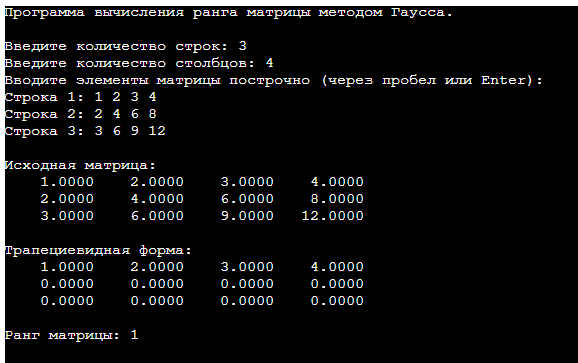
\includegraphics[width=0.8\textwidth]{screenshot.png}
    \caption{Результат выполнения программы (скриншот терминала)}\label{fig:screenshot}
\end{figure}

Скриншот с примером работы программы представлен на рис.~\ref{fig:screenshot}.



\begin{thebibliography}{9}
\bibitem{Knuth-2003}Кнут Д.Э. Всё про \TeX. \newblock --- Москва: Изд. Вильямс, 2003 г. 550~с.
\bibitem{Lvovsky-2003}Львовский С.М. Набор и верстка в системе \LaTeX{}. \newblock --- 3-е издание, исправленное и дополненное, 2003 г.
\bibitem{Voroncov-2005}Воронцов К.В. \LaTeX{} в примерах. 2005 г.
\end{thebibliography}

\end{document}